% ---------------------------------------
%
%  Renormalization and Running coupling constant
%  rge.tex
%  Program modified by Yasutoki Takamura
%  Last Modified Jan 22 2025
%
% ---------------------------------------
\section{走るゲージ結合定数}
場の量子論に基づけば, 理論に現れる発散を繰り込みという手法を用いて取り除くことが可能である.
%\textcolor{red}{種類などもう少し細かい説明をするか?}
繰り込みにはいくつかの手法があるが, いずれの方法であってもエネルギースケールへ依存性がある.
しかし理論はエネルギーの変化に対して不変でなければならないため, ラグランジアンに存在するパラメータはエネルギースケールの変化を打ち消すように変化する.
これによってエネルギースケールに依存する繰り込まれた理論が得られる.
\section{Callan-Symanzik方程式}
繰り込まれた量子場の理論ではラグランジアンの項は制限が与えられ, 質量次元が4次の項のみ許される.
繰り込まれた場の理論のパラメータは, 繰り込み条件の組みで決定され, この条件が繰り込みスケールを決定している.
異なるエネルギースケールであっても同様の理論を考えることができる.

繰り込み条件を考えると, 繰り込みを行うスケール$M$は任意である.
したがって, 同じ理論を異なったスケール$M'$でも定義することができる.
このことを以下で考える. 

ある理論のグリーン関数が
\begin{align}
  \langle T \phi_0(x_1)\cdots\phi_0(x_n)\rangle  \label{rescale1}
\end{align}
で与えられるとする.
この理論では, 量子効果を考えない裸の結合定数$\lambda_0$や, 運動量カットオフが$\Lambda$によって与えられるものであり,エネルギースケール$M$には依存していない.
エネルギースケール依存性は, このグリーン関数にあるのではなく, 場をリスケーリングし裸の結合定数$\lambda_0$を消して繰り込まれた結合定数$\lambda$で書くことでカットオフ依存性を取り除いたときにのみ現れる.
繰り込まれたグリーン関数と裸のグリーン関数は, リスケーリング因子の$Z$に至るまでは数値的に同じになる.
場の繰り込みは場の強さの繰り込み因子である$Z$を用いて次のように定義される.
\begin{align}
  \phi(x) = Z^{-\frac{1}{2}}\phi_0(x) \label{bfnc-2}
\end{align}
これにより繰り込まれた$n$点の相関関数は, 裸の相関関数と次のように関係付けられる.
\begin{align}
  \langle T \phi(x_1)\cdots \phi(x_n)\rangle = Z^{-\frac{n}{2}}\langle T \phi_0(x_1)\cdots \phi(x_n)\rangle \label{bfnc-1}
\end{align}
式(\ref{bfnc-1})の左辺は繰り込まれたグリーン関数と呼ばれる.
この関数は右辺のグリーン関数とは異なる別のエネルギースケールである$M'$で定義されており, 結合定数は$\lambda'$, リスケーリング因子は$Z'$で定義される.

ここから, エネルギースケール$M$を無限小だけシフトした場合の影響を考える.
はじめに$G^{(n)}(x_1,\cdots,x_n)$を繰り込まれた摂動論において計算される連結$n$点関数とする.
\begin{align}
  G^{(n)}(x_1,\cdots,x_n) = \langle T\phi(x_1)\cdots\phi(x_n) \rangle_{\text{connected}}\label{rnpf}
\end{align}
繰り込みされていない裸の相関関数は, 繰り込みされていないパラメータである$(\phi_0,\lambda_0,m_0)$とカットオフ$\Lambda$に依存している.
一方で, 繰り込まれた相関関数(式(\ref{rnpf}))には繰り込まれたパラメーターである($\phi,\lambda,m)$と繰り込みスケール$\mu$に依存している.
このことから, 繰り込みされていない裸の相関関数$G^{(n)}_0$は繰り込みスケール$\mu$に依存せず, 繰り込みスケールの変化があった場合でも変化することがないので
\begin{align}
  \frac{d G_0^{(n)}}{d\mu} = 0 \label{bfnc-3}
\end{align}
が満たされる.
一方で, 繰り込まれた相関関数は繰り込みスケールが変化することで影響を受ける.
繰り込みスケールを無限小だけシフトする.
\begin{align}
  \mu\quad\rightarrow\quad \mu + \delta \mu \label{sftM}
\end{align}
このとき, 繰り込みスケールの変化に伴って$\lambda$と$\phi$は次のように変化する.
\begin{align}
  &\lambda \quad\rightarrow\quad \lambda + \delta \lambda \label{sftl}\\
  &\phi \quad\rightarrow\quad \phi+ \delta\phi \equiv (1+\delta\eta)\phi \label{sftp}
\end{align}
場の変換については無次元のシフトを$\delta \eta  = \frac{\delta\phi}{\phi}$とした.
式(\ref{bfnc-2})から
\begin{align}
  Z^{\frac{1}{2}} = 1 - \delta\eta\label{bfnc-4}
\end{align}
が言えるので, 式(\ref{bfnc-3})から繰り込みされた相関関数は
\begin{align}
  G^{(n)}\quad\rightarrow\quad(1+n\delta\eta)G^{(n)}\label{sftg}
\end{align}
と変化することがわかる.
これらを踏まえて, 繰り込みされた相関関数の微小変化を考えると, 式(\ref{bfnc-3})から
\begin{align}
  \frac{d}{d\mu} Z^{\frac{n}{2}}G^{(n)} = \frac{\partial G^{(n)}}{\partial \mu} + \frac{\partial G^{(n)}}{\partial \lambda}\frac{\partial \lambda}{\partial \mu} - n \frac{\partial \eta}{\partial \mu}G^{(n)} = 0
\end{align}
がわかるので, これを整理して
\begin{align}
  \left(\mu \frac{\partial}{\partial \mu} + \mu\frac{\partial \lambda}{\partial \mu} \frac{\partial}{\partial \lambda} -n\mu\frac{\partial \eta}{\partial \mu}\right)G^{(n)}(x_1,\cdots,x_n;\mu,\lambda) = 0\label{CS-1}
\end{align}
となる.
ここで無次元の量である$\beta$と$\gamma$を
\begin{align}
  &\beta = \mu\frac{\partial \lambda}{\partial \mu}\label{def_beta}\\
  &\gamma = -\mu\frac{\partial \eta}{\partial \mu} \label{def_gamma}
\end{align}
と定義すると, 次の関係式が得られる.
\begin{align}
  \left(\mu \frac{\partial }{\partial \mu} + \beta \frac{\partial}{\partial \lambda} + n \gamma\right) G^{(n)}(x_1,\cdots,x_n;\mu,\lambda) = 0 \label{bfnc-CS1}
\end{align}
式(\ref{bfnc-CS1})はCallan-Symanzik方程式と呼ばれる. \cite{callanBrokenScaleInvariance1970,symanzikSmallDistanceBehaviour1970,symanzikSmalldistancebehaviourAnalysisWilson1971}

Callan-Symanzik方程式に現れる$\beta, \gamma$の2つの関数はカットオフスケールの$\Lambda$に依存し, 繰り込みスケール$\mu$に依存しない.
つまり, この$\beta, \gamma$の2つの関数は次元を持たない繰り込まれた結合定数である$\lambda$の関数であることが言える.
これらは$G^{(n)}$にのみ繰り込みが行われているからである.

ここで新しく定義された$\beta, \gamma$の2つの関数は不変的な関数であり, 繰り込み定数と場の強さの変化にのみ依存しており, これらが変化したときの繰り込みスケール$\mu$の変化を補うように変化が起こる. 
そのため$\beta$関数は繰り込みスケールが$\mu$への結合定数の依存性を表し, 一方で$\gamma$関数は場を繰り込みスケール$\mu$への依存性を表している

次にCallan-Symanzik方程式に現れた新たな関数$\gamma$をを一般化し, 摂動との関係を考える.
$\delta \eta$は式(\ref{sftp})で定義されていた.
したがって,
\begin{align}
  \delta \eta &= \frac{Z^{-\frac{1}{2}}(\mu+\delta \mu)}{Z^{-\frac{1}{2}}(\mu)}-1\nonumber\\
              &= \frac{Z^{-\frac{1}{2}}(\mu+\delta \mu)-Z^{-\frac{1}{2}}(\mu)}{Z^{-\frac{1}{2}}(\mu)}
\end{align}
となる.
この両辺を$\delta \mu$で割り, $\delta \mu\rightarrow0$とすると
\begin{align}
  \frac{\partial \eta}{\partial \mu} = -\frac{1}{2}\frac{1}{Z}\frac{\partial Z}{\partial \mu}
\end{align}
一方で$\gamma$は式(\ref{def_gamma})で定義されているので,
\begin{align}
  \gamma = \frac{1}{2}\frac{\mu}{Z} \frac{\partial Z}{\partial \mu}\label{def_gamma_correct}
\end{align}
と$\gamma$の表し方を変えることができる.
ここから摂動論の関係を見ることができる.
摂動論を考えているとき, 場の強さ$Z$は
\begin{align}
  Z = 1 +\delta Z
\end{align}
と微小量$\delta Z \ll 1$を用いて書くことができる.
これより
\begin{align}
  \gamma \simeq \frac{1}{2}\mu \frac{\partial \delta Z}{\partial \mu} + \mathcal{O}((\delta Z)^2)
\end{align}
となる.
このことから摂動論が有効な理論であれば, $\delta Z$が判明すれば 相殺項から体系的に$\beta$関数を求めることができることがわかる.

ここまではCallan-Symanzik方程式をスカラー場の理論として式(\ref{rescale1})から導出した.
一般にフェルミオン場が存在した場合でも成り立つ.
$n$個のフェルミオン場, $m$個のスカラー場が存在し, 両方の結合定数が$\lambda$の場合を考える.
このとき, 場のくりこみを同じように考えると, 繰り込まれたグリーン関数は
\begin{align}
  G_0^{(n,m)}(\{x_i\},\lambda_0) = Z_\psi^{\frac{n}{2}} Z_\phi^{\frac{m}{2}}G^{(n,m)}(\{x_i\},\lambda,\mu)\label{renormalized_G}
\end{align}
となる.
したがって, 式(\ref{bfnc-3})と同じように考えて
\begin{align}
  \left(\mu\frac{\partial}{\partial \mu} + \beta\frac{\partial}{\partial \lambda} + n\gamma_\psi + m \gamma_\phi \right)G^{(n,m)}(\{x_i\},\mu,\lambda) = 0\label{renormalized_CS}
\end{align}
となる.
ここでは
\begin{align}
  \gamma_\psi = \frac{n}{2}\frac{\mu}{Z_\psi}\frac{\partial Z_\psi}{\partial \mu},\quad \gamma_\phi = \frac{m}{2}\frac{\mu}{Z_\phi}\frac{\partial Z_\phi}{\partial \mu}\label{def_gamma2}
\end{align}
とした.

これらより, 式(\ref{def_beta})
\begin{align}
  \beta \equiv \mu\frac{\partial}{\partial \mu}\lambda\nonumber
\end{align}
の$\beta$からゲージ結合定数$\lambda$のエネルギー依存性を求めることができる.
この$\beta$は摂動論において相殺項や繰り込まれたグリーン関数から求めることができ, 非可換ゲージ理論や湯川結合, スカラー場の理論など一般的な場の理論で同様に求めることができる.
\cite{chengHiggsPhenomenaAsymptotically1974,
machacekFermionHiggsMasses1981,
machacekTwoloopRenormalizationGroup1983,
machacekTwoloopRenormalizationGroup1984,
machacekTwoloopRenormalizationGroup1985,
maVariationMixingAngles1979,
vaughnRenormalizationGroupConstraints1982}
\section{ゲージ結合定数のエネルギー依存性}
式(\ref{def_beta})により, ゲージ結合定数のエネルギー依存性を$\beta$関数によって導くことができることが明らかにされた.
理論に現れる相殺項を求めることで$\beta$-関数の具体的な形を求めることができるが, 群論の対称性を用いることで一般的な$\beta$-関数の係数は導出されている.
摂動の$\delta Z$の1次の影響まで考えた場合,
\begin{align}
  \beta = -\frac{g^3}{(4\pi)^2}\left[\frac{11}{3}C_2(G) -\frac{4}{3}\kappa S(F) - \frac{1}{6}\eta S(S)\right]
\end{align}
となる.
\footnote{
本論文では扱わないが, 2次までの摂動の計算をすると次のようになる.
\cite{caswellAsymptoticBehaviorNonAbelian1974,jonesTwoloopDiagramsYangMills1974,jonesTwoLoopBeta1982}
\begin{align}
  \beta &= -\frac{g^3}{(4\pi)^2}\left[\frac{11}{3}C_2(G) -\frac{4}{3}\kappa S_2(F) - \frac{1}{6}\eta S_2(S)\right] \nonumber\\
        &\quad-\frac{g^5}{(4\pi)^4}\left[ \frac{34}{3}[C_2(G)]^2 -\kappa\left(4C_2(F)+\frac{20}{3}C_2(G)\right)S_2(F) -\left(2C_2(S)+\frac{1}{3}C_2(G)\right)\eta S_2(S)\right] \nonumber
\end{align}
}
\cite{grossUltravioletBehaviorNonAbelian1973,politzerReliablePerturbativeResults1973}

多重項は群$G$の表現$R$によって変換される.
ここではフェルミオン多重項であれば群$G$の表現$F$によって, ボゾン多重項は群$G$の表現$S$によって変換する.
ここでは,$C_2(R)$は
$\kappa$ $\eta$はそれぞれ
\begin{align}
  \kappa = \left\{\begin{array}{cc}
      1 & ディラックフェルミオン \\
      \cfrac{1}{2} & ワイルフェルミオン
    \end{array}\right.,\quad
  \eta = \left\{\begin{array}{cc}
      1 & 実スカラー場\\
      2 & 複素スカラー場
    \end{array}\right. \nonumber
\end{align}
と対応づけられる.
また, $S_2(F), S_2(S)$はそれぞれフェルミオン表現とスカラー表現のDynkin指数である.
群$G$の生成子の表現行列を$T^a$とする.
これは交換関係(\ref{gauge-1})を満たす.
この表現行列$T^a$は次の関係を満たす.
\begin{align}
  T^a T^a &= C_2(R)I\nonumber\\
  \mathrm{Tr}[T^a T^b] &= S_2(R)\delta^{ab}\nonumber
\end{align}
ここで$I$は単位行列である.
$C_2(R)$はカシミア演算子と呼ばれ, 群$G$の生成子と交換する.
\begin{align}
  d(G)S_2(R) = d(R)C_2(R)
\end{align}
ここで, $d(R)$は$R$の次元であり, $d(G)$はゲージ群$G$の随伴表現の次元である.
随伴表現の次元は群の次元と等しい.

ここで$b_i$を
\begin{align}
  b_i &= -\frac{11}{3}C_2(G) +\frac{4}{3}\kappa S_2(F) + \frac{1}{6}\eta S_2(S)\nonumber
\end{align}
とし, $i=1,2,3$はそれぞれ$U(1)_Y, SU(2)_L, SU(3)_c$ゲージ群と対応する.
また, 後述される式(\ref{re_gY})によって$U(1)_Y$ゲージ結合定数は$g_1^2\equiv \sqrt{\frac{5}{3}}g_Y$と規格化される.
標準模型では
\begin{align}
  \left(b_1, b_2, b_3 \right) = \left( \frac{41}{10}, -\frac{19}{6}, -7\right)\nonumber
\end{align}
と係数を求めることができる\footnote{求め方は付録Bに掲載した}.
ここから実際に数値的にゲージ結合定数の大きさについて, エネルギー依存性を見る.
\begin{figure}[ht]
  \centering
  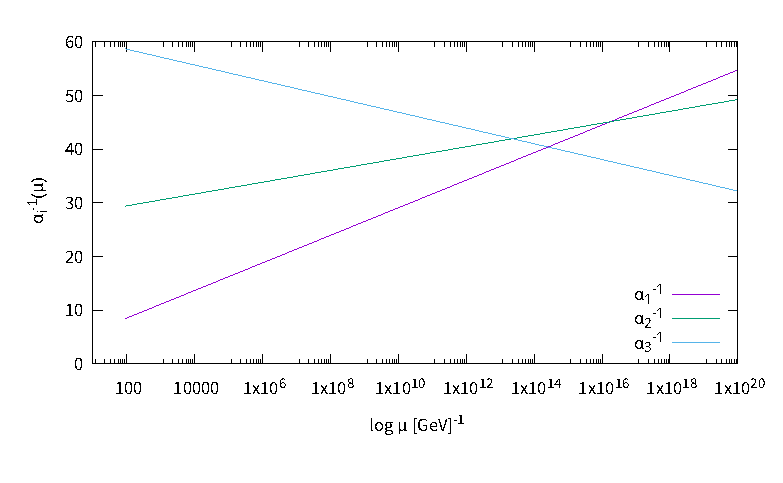
\includegraphics[width=12truecm,clip]{fig/RGE_SM.eps}
  \caption{標準模型粒子のみで繰り込み群方程式を解いた図}
  \label{fig:RGE_SM}
\end{figure}
$\alpha_i$は$\alpha_i(\mu) = \cfrac{g_i(\mu)}{4\pi}$として, 式(\ref{def_beta})に代入し, 
\begin{align}
  \frac{d \alpha_i^{-1}(\mu)}{d\,\mathrm{ln}{\mu}} = -\frac{1}{2\pi}b_i \label{bfnc_1loop}
\end{align}
とする.
電弱スケール $M_Z=91.1880\,[\mathrm{GeV}]$におけるゲージ結合定数の値は
\begin{align}
  g_1(M_Z) &= 0.461\nonumber\\
  g_2(M_Z) &= 0.652\nonumber\\
  g_3(M_Z) &= 1.22\nonumber
\end{align}
であり
\cite{navasReviewParticlePhysics2024}, これらを初期条件として数値的に解いたものが図\ref{fig:RGE_SM}となる.
図\ref{fig:RGE_SM}を見ると明らかであるが, 高エネルギースケールでゲージ結合定数の大きさは近づくものの, 完全には一致しない.
しかし, いずれの相互作用の大きさもプランクスケールである$M_{pl}\sim 10^{19}\,[\mathrm{GeV}]$よりも下で近づくため, 3つの相互作用は重力相互作用よりも先に統一される可能性は残されている.

%EOF
